\documentclass[12pt, a4paper]{book}%, oneside

\usepackage[headings]{fullpage}
\usepackage{setspace}

% \usepackage[top=1.5cm,right=1.5cm,bottom=1.5cm,left=1.5cm]{geometry}
% \usepackage{fancyhdr}
% \setlength{\headheight}{20pt} 
% \usepackage{graphics}
\usepackage{graphicx}
\usepackage{float}
\usepackage{subfig}
\usepackage{amsthm}
\usepackage{amsmath}
\usepackage{amssymb}
\usepackage{amsfonts}
\usepackage{mathrsfs}
\usepackage{array}
% \usepackage{xtab}
\usepackage{multirow}
\usepackage{booktabs}
\usepackage{appendix}
\usepackage[pdfborder={0 0 0}, colorlinks=true, linkcolor=black, citecolor=blue]{hyperref}
\usepackage[printonlyused]{acronym}
\usepackage{algorithmic}
\usepackage{algorithm}
\usepackage{ifpdf}
\usepackage[utf8]{inputenc}
\usepackage{textcomp}
\usepackage{enumitem}
\usepackage{dsfont}
\usepackage{stmaryrd}
\usepackage{tikz}
\usepackage{venndiagram}
\usepackage{tcolorbox}
\usepackage{float}
\usepackage{urwchancal}


\setlength{\parindent}{0pt}

\newcommand{\submissionDay}{1}
\newcommand{\submissionMonth}{July}
\newcommand{\submissionYear}{2023}
\newcommand{\submissionDate}{\submissionDay~\submissionMonth,~\submissionYear}
\newcommand{\typeOfThesis}{Bachelor Thesis}
%
\newcommand{\titleOfThesisOne}{Adding Events to $Log_AS$}
%
\newcommand{\authorOfThesis}{Ibrahim Abou Elenein}
\newcommand{\supervisorOne}{Prof Haythem Ismail}
%     \begin{figure}[ht]
%      \centering
%       \includegraphics[width=#1\textwidth]{images/#2}
%       \caption{#3}
%       \label{#4}
%     \end{figure}
% }
%
% \newcommand{\includefigWSC}[5]{
%     \begin{figure}[ht]
%      \centering
%       \includegraphics[width=#1\textwidth]{images/#2}
%       \caption[#3]{#4}
%       \label{#5}
%     \end{figure}
% }
%
% \newcommand{\includeeps}[4]{
% \includefig{#1}{#2.eps}{#3}{#4}
% }
%
% \newcommand{\includeepsWSC}[5]{
% \includefigWSC{#1}{#2.eps}{#3}{#4}{#5}
% }
%
\theoremstyle{definition}
\newtheorem{exmp}{Example}[section]
\newtheorem{defn}{Definition}[section]
\newtheorem{axiom}{Axiom}[section]
\newtheorem{theorem}{Theorem}[section]
\newtheorem{lemma}{Lemma}[section]
\newtheorem{prop}{Proposition}[section]
% proof environment with a small square as a "qed" symbol
% \renewenvironment{proof}[1][Proof]{\begin{trivlist} \item[\hskip \labelsep {\bfseries #1}]}{\hfill$\blacksquare$\end{trivlist}}




\ifpdf
\pdfinfo {
	/Author (\authorOfThesis)
	/Title (\titleOfThesisOne)
	/Subject (\typeOfThesis)
	/Keywords ()
	/CreationDate (D:20090707085533)
}
\fi

\begin{document}
\overfullrule=5pt
\pagestyle{plain}
\pagenumbering{Roman}

\include{GUC_TitlePage}

\chapter*{Acknowledgments}
\addcontentsline{toc}{chapter}{Acknowledgments}
\label{chap:ack}

I express my deepest gratitude to my esteemed supervisor, Prof Haythem Ismail, whose unwavering support and guidance were instrumental in the success of my bachelor's thesis. His vast knowledge, patience, and motivation helped me navigate the research and writing process, enabling me to achieve excellence in my work. I am fortunate to have had such an exceptional mentor, and I will always be grateful for his invaluable contributions to my academic journey.\\

I extend my heartfelt appreciation to my friends, who have supported and encouraged me throughout my academic endeavors. I want to give a special thanks to Arwa Ghoniem, who graciously took the time to read my thesis and provided me with insightful feedback and suggestions.\\

Lastly, I want to thank my family, including my mother, father, Mohammed, Mahmoud, and relatives. Your unwavering support and encouragement have driven my success, and I am grateful for your belief in me.
% write to mom and dad in italics
\label{chap:dedication}

\begin{center}
    \textit{To Mom and Dad}
\end{center}

\chapter*{Abstract}
\addcontentsline{toc}{chapter}{Abstract}
\label{chap:abstract}

In this study, I introduce $Log_A$T, a comprehensive family of languages specifically developed for the purpose of reasoning about temporal ontologies,
with a particular focus on states and events.
This innovative framework goes beyond the limitations of traditional languages by adopting a purely term-based approach,
rendering $Log_A$T an algebraic language.

The primary objective of this thesis is to delve into the analysis and understanding of punctual and durative events within the context of $Log_A$T.
By thoroughly investigating these event types, I aim to provide valuable insights into their representation and integration within the framework.
This research endeavor serves as a significant extension to the existing $Log_A$S language, as it allows for the seamless incorporation and reasoning of events alongside states.

Furthermore, this study addresses the crucial task of establishing a comprehensive framework that accounts for the intricacies of events. By carefully examining the relationships between events and states, this research aims to contribute to the development of an enriched $Log_A$S language that can effectively capture and reason about the dynamic nature of events.

By expanding the scope and capabilities of $Log_A$S through the introduction of $Log_A$T, this research strives to provide a valuable contribution to the field of temporal ontologies.
Through the exploration and analysis of punctual and durative events, this study not only enhances our understanding of these concepts but also enables more sophisticated and comprehensive reasoning within the extended $Log_A$S framework.
\tableofcontents
\addcontentsline{toc}{chapter}{Contents}
\clearpage

\pagestyle{headings}
\pagenumbering{arabic}

% \setlength\parskip{15pt}
\setlength\parskip{.5\baselineskip plus .2\baselineskip
	minus .4\baselineskip}
% \setlength\parskip{.5\baselineskip \@plus .1\baselineskip \@minus ..1\baselineskip}


% \include{introduction}
% \include{background}

% % add more chapters here

% \chapter*{Conclusion}
\addcontentsline{toc}{chapter}{Conclusion}


In extending the ontology of events, I have taken a simple and straightforward approach by augmenting the existing $Log_A$S language.
Within this enriched ontology, I have carefully considered and delineated two fundamental types of events: punctual events and durative events. These categories allow for a comprehensive understanding of various temporal phenomena.

A key aspect of my research involves exploring the intricate relationship between events and states.
By examining how events induce changes in states, I aim to elucidate the intricate dynamics and interdependencies that govern the temporal progression of systems. Through this analysis, I unveil the underlying mechanisms through which events shape and transform states.

Additionally, I delve into the realm of inference, showcasing how events can be inferred from the observable changes in states.
By establishing connections between state alterations and corresponding events, I offer insights into the deductive aspects of temporal ontologies.
This inference mechanism not only provides a deeper comprehension of the causal relationships between events and states but also enables the extraction of valuable information from observed changes.

By expanding the scope of $Log_A$S and incorporating these insights into my research, I seek to contribute to the development of a more comprehensive and robust framework for reasoning about temporal ontologies. Ultimately, this endeavor aims to enhance our understanding of events, states, and their intricate interactions, enabling more sophisticated analyses and applications in various domains.
\chapter{States and Events}
\section{Verbs and Time}
\subsection{Introduction}

In his paper ``Verbs and Time'' \cite{vendler1957verbs}, Vendler proposes a categorization of verbs based on their temporal and aspectual properties. The goal of this categorization is to provide a framework for understanding how verbs relate to time and how their meanings are structured.

\subsection{Background}

Verbs are a central component of natural language and are used to express actions, states, and events. They are also crucial for representing the temporal structure of sentences, as they allow us to talk about past, present, and future events. However, not all verbs are the same when it comes to their temporal properties. Some verbs, like ``run'' or ``sing'', describe actions that occur over a period of time, while others, like ``know'' or ``believe'', describe states or attitudes that hold at a particular point in time.

\subsection{Vendler's Categorization}

Vendler proposes a categorization of verbs based on their temporal and aspectual properties. He identifies four main categories of verbs: \textit{activities}, \textit{accomplishments}, \textit{achievements}, and \textit{states}.

\textbf{Activities} are verbs that describe ongoing processes or actions that have no inherent endpoint. Examples of activities include ``run'', ``swim'', and ``write''.


\textbf{Accomplishments} are verbs that describe actions that have a clear endpoint or goal. Examples of accomplishments include ``build'', ``solve'', and ``paint''.


\textbf{Achievements} are verbs that describe events that happen suddenly or instantaneously, without any inherent duration. Examples of achievements include ``win'', ``die'', and ``arrive''.


\textbf{States} are verbs that describe conditions or states of being that hold over a period of time. Examples of states include ``know'', ``believe'', and ``love''.

Each of these categories has a different temporal and aspectual structure, and Vendler argues that these differences are crucial for understanding the meaning of verbs and their relationships to time.



\begin{exmp} Analysis of the verb ``think''
  \begin{enumerate}
    \item He is ``thinking'' about John. \label{first}
    \item He ``thinks'' that John is a philosopher. \label{second}
  \end{enumerate}

  The verb ``think'' functions differently in the two sentences presented. In the first sentence \ref{first}, ``thinking'' is characterized as a \textit{process} that involves ongoing mental activity related to John, whereas in the second sentence \ref{second}, ``thinks'' describes a \textit{state} of belief or opinion about John.

  The first sentence \ref{first} suggests that the activity of ``thinking'' about something is a deliberate and continuous process that occurs over time. The phrase ``deliberately'' highlights the intentional nature of the activity. Furthermore, if one were to think about John for a period of time, it would imply that the thinking was consistent and continuous throughout that time period. This notion is expressed as \textit{homogeneity}.
\end{exmp}


\section{Interval Algebra}

Allen's paper presents a framework called the \textit{Interval Algebra} for representing and reasoning about actions and time in natural language processing and artificial intelligence systems \cite{allen1984towards}. The Interval Algebra uses a set of basic temporal relations to describe the temporal and causal relationships between events and actions. For example, it can represent relations such as ``before'',``after'',``meets'',``overlaps'',``during'', and ``equals'' between different intervals of time.

Allen argues that the Interval Algebra can be used to model a wide range of natural language expressions involving \textit{actions} and \textit{events}. This includes simple statements about temporal order, such as ``John ate breakfast before he went to work'', as well as more complex descriptions of causality and concurrency, such as ``When John opened the door, the alarm went off.''


\pagebreak
The logic used is a typed first-order logic.

\begin{exmp} Allen's Interval Algebra

  \begin{enumerate}
    \item DURING($t_1$, $t_2$) time interval $t_1$ is fully contained within time interval $t_2$.

    \item STARTS($t_1$, $t_2$) time interval $t_1$ shares a starting point with time interval $t_2$ but ends before $t_2$.

    \item FINISHES($t_1$, $t_2$) time interval $t_1$ shares the same end as time interval $t_2$ but starts after $t_2$.

    \item IN($t_1$, $t_2$) $\iff$ (DURING($t_1$, $t_2$) $\lor$ STARTS($t_1$, $t_2$) $\lor$ FINISHES($t_1$, $t_2$)). 

    \item HOLDS(\(\phi\), \(t\)) is true iff \(\phi\) holds during \(t\).
  \end{enumerate}



  \begin{center}
    HOLDS(\(\phi\), \(T\)) \(\iff ( \forall t \) IN $ (t,T) \implies $ HOLDS($\phi, t$)).
  \end{center}

  This definition states that HOLDS($\phi$, $T$) is true iff $\phi$ holds during every subinterval $t$ of $T$. In other words, $\phi$ holds throughout the entire interval $T$.
\end{exmp}

\subsection{Occurrences}
Allen uses three basic entities that are associated with time which are: \textit{properties}, \textit{events}, and \textit{processes}.
\begin{enumerate}
  \item \textbf{Events} describe an activity that involves an outcome. Examples of events such as ``John walked to the store''.

  \item \textbf{Processes} refer to some activity not associated with a result. Examples of processes include ``John was walking'' and ``John was running''.

  \item \textbf{Properties} are conditions that hold over a period of time. Examples of properties include ``John owns a cat''.
\end{enumerate}
One way to distinguish between \textit{events} and \textit{processes} is that one can count how many times an event occurs, but one cannot count 
the number of times a process occurs.


The predicate OCCUR takes an event and a time interval and is true if the event happens over the time interval $t$ and there is no subinterval of $t$
over which the event occurs.

\begin{center}
  OCCUR($e$, $t$) $\land$ IN($t^\prime$, $t$) $\implies$ \(\lnot\) OCCUR($e$, $t^\prime$).
\end{center}

Another way is to consider the characteristics of the set of temporal intervals that they hold or occur over. 
consider the \textit{process} ``I am walking'' over the Interval $I$. Unlike \textit{events}, this process might be occurring over subintervals of $I$ however a \textit{property} must be holding over every subinterval of $I$.


If a process $p$ took place over interval $t$ is denoted by the formula OCCURRING$(p,t)$.


As we illustrated, a process occurring over an interval $T$, must be occurring over at least one subinterval of $T$.

\section{Shoham and Allen's Temporal Logic}

In his paper ``Temporal Logics in AI: Semantical and Ontological Considerations,''\cite{shoham1988temporal}. 
Shoham shows how Allen' Ontology have a problem defining the properties as they are not only not precise but they look like the FOPC, so he missed the-off-shelf FOPC.

Also he shows that Allen's Ontology introduces unnecessary complexity just because Allen went for using intervals instead of time points.

Shoham also the distinction between \textit{properties}, \textit{events}, and \textit{processes} is unnecessary and it's not very useful.


\subsection{Shoham's Interval Logic}
\subsubsection{Syntax}
\begin{itemize}
  \item Given $TC$ a set of time points symbols,
  \item $C$ a set of constant symbols that's disjoint from $TC$;
  \item $TV$ a set of temproal variables,
  \item $V$ a set of variables that's disjoint from $TV$. 
  \item $TF$ a set of temporal function symbols,
  \item $F$ a set of function symbols that's disjoint from $TF$.
  \item $R$ a set of relation symbols.
\end{itemize}

The set of temporal formulas is defined inductively as follows:
\begin{enumerate}
  \item All members of $TC$ are temporal terms.
  \item All members of $TV$ are temporal terms.
  \item if $trm_1, \dots, trm_n$ are temporal terms, and $f \in TF$ is an $n$-ary temporal function symbol, then $f(trm_1, \dots, trm_n)$ is a temporal term.
\end{enumerate}

The set of \textit{nontemporal formulas} is defined inductively in exactly the same way as the set of temporal formulas, with 
$TC$ replace by $C$, $TV$ replaced by $V$, $TF$ replaced by $F$.

The set of well-formed formulas (wffs) is defined inductively as follows:
\begin{enumerate}
  \item if $trm_a$ and $trm_b$ are temporal terms, then $trm_a = trm_b$ and $trm_a \preceq trm_b$ are wffs.
  \item if $trm_a$ and $trm_b$ are temporal terms, $trm_1, \dots, trm_n$ are non-temporal terms, and $r \in R$ are n-ary relation symbol,
    then 
    \[
      \text{TRUE}(trm_a, trm_b, r(trm_1, \dots, trm_n))
    \]
    is a wff.
  \item if $\phi_1$ and $\phi_2$ are wffs, then $\phi_1 \land \phi_2$ and $\neg \phi_1$ are wffs.
  \item if $\phi$ is a wff and $z \in TV \cup V$ is a variable, then $\forall z \phi$ is a wff.
\end{enumerate}

Again, we assume the usual definition of $\lor, \exists, \equiv, \supset$ and so on. 

\begin{exmp} Here's an example sentences.
  \begin{equation}
    \text{TRUE}(t_1, t_2, \text{COLOR}(\text{HOUSE17}, \text{RED})))
  \end{equation}
  \begin{equation}
  \exists u \ \text{TRUE}(t_3, t_4, \text{ON}(u,B))
  \end{equation}
\end{exmp}

\subsubsection{Semantics}
An \textit{interpretation} is a tuple $\mathscr{S} = \langle  TW,\ \leqslant,\ W,\ TFN,\ FN,\ RL,\ M\rangle$ where $TW$ 
is a nonempty universe of time points, $\leqslant$ is a binary relation on $TW$, $W$ is a nonempty universe of individuals,
that is disjoint from $TW$, $TFN$ is a set of total functions $\bigcup_k (TW^k \rightarrow TW)$, 
$FN$ is a set of total functions $ \bigcup_k (W^k \rightarrow W)$, $RL$ is a set of total relations over $W$, and 
$M = \langle M1,\ M2,\ M3,\ M4,\ M5 \rangle$ is a meaning function as follows: $M_1 : T \rightarrow TW$,
$M_2: C \to W$, $M_3 : TF \to TFN$, $M_4 : TW \times TW \times F \to FN$, and $M_5: TW \times TW \times R \to RL$

A \textit{variable assignment} is a function $ VA = \langle VAT,\ VAV \rangle$, such that $VAT: VT \to TW$ and 
$VAV: V \to W$. $M$ and $VA$ induce a time-dependent meaning $MVA$ on arbitrary terms in the following way.

We first define the meaning of arbitrary temporal terms. That meaning is the same regardless of when the terms are interpreted: the terms $1.1.2000$ and
$(12:00 + 12_{min})$ each denote a single, unambiguous absolute time. The precise
meaning of temporal terms is as follows. If $vt \in VT $, then $MVA (vt) = VAT (vt)$.
If $ct \in CT$, then $MVA (ct) = M_1(ct)$. If $f \in T F$ and $trm = f(trm_1, . . . , trm_n)$ Is a
temporal term, then
\[
  MVA(trm) = M_3(f)(MVA(trm_1), \dots, MVA(trm_n))
\]

\pagebreak

\section{Galton and Allen's Temporal Logic}
In his paper ``A Critical Examination of Allen's
Theory of Action and Time''\cite{galton2004}, Galton shows that Allen's Ontology is unsuitable for representing facts and continuous change.

\chapter{Temporal Representation and Reasoning}
\label{ch:states-and-events}
In this chapter, we will take a look at previous work on temporal representation and reasoning.


\section{Vendler's Categorization}

In his paper \cite{vendler1957verbs}, Vendler proposes a categorization of verbs based on their temporal and aspectual properties. The goal of this categorization is to provide a framework for understanding how verbs relate to time and how their meanings are structured.

Verbs are a central component of natural language and are used to express actions, states, and events. They are also crucial for representing the temporal structure of sentences, as they allow us to talk about past, present, and future events. However, not all verbs are the same when it comes to their temporal properties. Some verbs, like ``run'' or ``sing'', describe actions that occur over a period of time, while others, like ``know'' or ``believe'', describe states or attitudes that hold at a particular point in time.


Vendler proposes a categorization of verbs based on their temporal and aspectual properties. He identifies four main categories of verbs: \textit{activities}, \textit{accomplishments}, \textit{achievements}, and \textit{states}.

\textbf{Activities} are verbs that describe ongoing processes or actions that have no inherent endpoint. Examples of activities include ``run'', ``swim'', and ``write''.


\textbf{Accomplishments} are verbs that describe actions that have a clear endpoint or goal. Examples of accomplishments include ``build'', ``solve'', and ``paint''.


\textbf{Achievements} are verbs that describe events that happen suddenly or instantaneously, without any inherent duration. Examples of achievements include ``win'', ``die'', and ``arrive''.


\textbf{States} are verbs that describe conditions or states of being that hold over a period of time. Examples of states include ``know'', ``believe'', and ``love''.

Each of these categories has a different temporal and aspectual structure, and Vendler argues that these differences are crucial for understanding the meaning of verbs and their relationships to time.



\begin{exmp} Analysis of the verb ``think''
	\begin{enumerate}
		\item He is ``thinking'' about John. \label{first}
		\item He ``thinks'' that John is a philosopher. \label{second}
	\end{enumerate}

	The verb ``think'' functions differently in the two sentences presented. In the first sentence \ref{first}, ``thinking'' is characterized as a \textit{process} that involves ongoing mental activity related to John, whereas in the second sentence \ref{second}, ``thinks'' describes a \textit{state} of belief or opinion about John.

	The first sentence \ref{first} suggests that the activity of ``thinking'' about something is a deliberate and continuous process that occurs over time. The phrase ``deliberately'' highlights the intentional nature of the activity. Furthermore, if one were to think about John for a period of time, it would imply that the thinking was consistent and continuous throughout that time period. This notion is expressed as \textit{homogeneity}.
\end{exmp}


\section{Interval Algebra}

Allen's paper presents a framework called the \textit{Interval Algebra} for representing and reasoning about actions and time in natural language processing and artificial intelligence systems \cite{allen1984towards}. The Interval Algebra uses a set of basic temporal relations to describe the temporal and causal relationships between events and actions. For example, it can represent relations such as ``before'',``after'',``meets'',``overlaps'',``during'', and ``equals'' between different intervals of time.

Allen argues that the Interval Algebra can be used to model a wide range of natural language expressions involving \textit{actions} and \textit{events}. This includes simple statements about temporal order, such as ``John ate breakfast before he went to work'', as well as more complex descriptions of causality and concurrency, such as ``When John opened the door, the alarm went off.''

Allen presents a \textit{many-sorted} \textit{first-order} logic, defining several sorts related to various ontological entities identified.

Allen takes the \textit{interval} as the temporal primitive, completely excluding the notion of \textit{point} from the theory, arguing that our direct experience
is with events and actions which typically take time to occur.

He Introduced a set of 13 mutually exclusive binary relations between intervals and
defined the \textit{interval algebra} as all the possible disjunctions that can be formed from these relations.

In this framework, time is modeled as \textit{linear} and \textit{infinite}, the interval structure implies time is \textit{continuous}.

\begin{exmp} Allen's Interval Algebra

	\begin{enumerate}
		\item DURING($t_1$, $t_2$) time interval $t_1$ is fully contained within time interval $t_2$.

		\item STARTS($t_1$, $t_2$) time interval $t_1$ shares a starting point with time interval $t_2$ but ends before $t_2$.

		\item FINISHES($t_1$, $t_2$) time interval $t_1$ shares the same end as time interval $t_2$ but starts after $t_2$.

		\item IN($t_1$, $t_2$) $\iff$ (DURING($t_1$, $t_2$) $\lor$ STARTS($t_1$, $t_2$) $\lor$ FINISHES($t_1$, $t_2$)).

		\item HOLDS(\(\phi\), \(t\)) is true iff \(\phi\) holds during \(t\).
	\end{enumerate}



	\begin{center}
		HOLDS(\(\phi\), \(T\)) \(\iff ( \forall t \) IN $ (t,T) \implies $ HOLDS($\phi, t$)).
	\end{center}

	This definition states that HOLDS($\phi$, $T$) is true iff $\phi$ holds during every subinterval $t$ of $T$. In other words, $\phi$ holds throughout the entire interval $T$.
\end{exmp}

\begin{exmp} Complex logical expressions

	To allow properties to name complex logical expressions, there is a set of
	functions \textit{and}, \textit{or}, \textit{not}, \textit{all}, \textit{and} \textit{exists}, that correspond to the logical operators
	$\&, \lor, \sim, \forall$ and $\exists$ respectively.
	Conjunction moves through the HOLDS predicate freely:
	\begin{equation}
		\text{HOLDS}(\text{and}(p, q), t) \iff \text{HOLDS}(p, t) \  \& \  \text{HOLDS}(q, t)
	\end{equation}

	Negation is defined as follows:
	\begin{equation}
		\text{HOLDS}(\text{not}(p), T) \iff (\forall t.\text{IN}(t, T) \implies \sim \text{HOLDS}(p, t))
	\end{equation}
\end{exmp}




\subsection{Occurrences}
Allen uses three basic entities that are associated with time which are: \textit{properties}, \textit{events}, and \textit{processes}.
\begin{enumerate}
	\item \textbf{Events} describe an activity that involves an outcome. Examples of events such as ``John walked to the store''.

	\item \textbf{Processes} refer to some activity not associated with a result. Examples of processes include ``John was walking'' and ``John was running''.

	\item \textbf{Properties} are conditions that hold over a period of time. Examples of properties include ``John owns a cat''.
\end{enumerate}
One way to distinguish between \textit{events} and \textit{processes} is that one can count how many times an event occurs, but one cannot count
the number of times a process occurs.


The predicate OCCUR takes an event and a time interval and is true if the event happens over the time interval $t$ and there is no subinterval of $t$
over which the event occurs.

\begin{center}
	OCCUR($e$, $t$) $\land$ IN($t^\prime$, $t$) $\implies$ \(\lnot\) OCCUR($e$, $t^\prime$).
\end{center}

Another way is to consider the characteristics of the set of temporal intervals that they hold or occur over.
Consider the \textit{process} ``I am walking'' over the Interval $I$. Unlike \textit{events}, this process might be occurring over subintervals of $I$ however a \textit{property} must be holding over every subinterval of $I$.


If a process $p$ took place over interval $t$ is denoted by the formula OCCURRING$(p,t)$.


As we illustrated, a process occurring over an interval $T$, must be occurring over at least one subinterval of $T$.

\section{Shoham Temporal Logic}

In his paper \cite{shoham1988temporal}.
Shoham shows how Allen' Ontology have a problem defining the properties as they are not only not precise but they look like the $\mathcal{FOPC}$, so he missed the-off-shelf $\mathcal{FOPC}$.

Also he shows that Allen's Ontology introduces unnecessary complexity just because Allen went for using intervals instead of time points.

Shoham also the distinction between \textit{properties}, \textit{events}, and \textit{processes} is unnecessary and it's not very useful.
For example, much of Allen's discussion of event causation, ECAUSE, should apply to pairs of properties and mixed pairs of properties and events. Furthermore, this distinction is insufficient to express some other properties of propositions, such as that if a proposition holds over two overlapping intervals then it holds over
the union of the two intervals, though not necessarily vice versa (``I ran for more than two mile'').


\subsection{Shoham's Interval Logic}
Shoham has proposed the use of \textit{points} rather than \textit{intervals} as the basic temporal element and defines an interval as a pair of points.
\subsubsection{Syntax}
\begin{itemize}
	\item Given $TC$ a set of time points symbols,
	\item $C$ a set of constant symbols that's disjoint from $TC$;
	\item $TV$ a set of temproal variables,
	\item $V$ a set of variables that's disjoint from $TV$.
	\item $TF$ a set of temporal function symbols,
	\item $F$ a set of function symbols that's disjoint from $TF$.
	\item $R$ a set of relation symbols.
\end{itemize}

The set of temporal formulas is defined inductively as follows:
\begin{enumerate}
	\item All members of $TC$ are temporal terms.
	\item All members of $TV$ are temporal terms.
	\item if $trm_1, \dots, trm_n$ are temporal terms, and $f \in TF$ is an $n$-ary temporal function symbol, then $f(trm_1, \dots, trm_n)$ is a temporal term.
\end{enumerate}

The set of \textit{nontemporal formulas} is defined inductively in exactly the same way as the set of temporal formulas, with
$TC$ replace by $C$, $TV$ replaced by $V$, $TF$ replaced by $F$.

The set of well-formed formulas (wffs) is defined inductively as follows:
\begin{enumerate}
	\item if $trm_a$ and $trm_b$ are temporal terms, then $trm_a = trm_b$ and $trm_a \preceq trm_b$ are wffs.
	\item if $trm_a$ and $trm_b$ are temporal terms, $trm_1, \dots, trm_n$ are non-temporal terms, and $r \in R$ are n-ary relation symbol,
	      then
	      \[
		      \text{TRUE}(trm_a, trm_b, r(trm_1, \dots, trm_n))
	      \]
	      is a wff.
	\item if $\phi_1$ and $\phi_2$ are wffs, then $\phi_1 \land \phi_2$ and $\neg \phi_1$ are wffs.
	\item if $\phi$ is a wff and $z \in TV \cup V$ is a variable, then $\forall z \phi$ is a wff.
\end{enumerate}

Again, we assume the usual definition of $\lor, \exists, \equiv, \supset$ and so on.

\begin{exmp} Here's an example sentences.
	\begin{equation}
		\text{TRUE}(t_1, t_2, \text{COLOR}(\text{HOUSE17}, \text{RED})))
	\end{equation}
	\begin{equation}
		\exists u \ \text{TRUE}(t_3, t_4, \text{ON}(u,B))
	\end{equation}
\end{exmp}

\subsubsection{Semantics}
An \textit{interpretation} is a tuple $\mathscr{S} = \langle  TW,\ \leqslant,\ W,\ TFN,\ FN,\ RL,\ M\rangle$ where $TW$
is a nonempty universe of time points, $\leqslant$ is a binary relation on $TW$, $W$ is a nonempty universe of individuals,
that is disjoint from $TW$, $TFN$ is a set of total functions $\bigcup_k (TW^k \rightarrow TW)$,
$FN$ is a set of total functions $ \bigcup_k (W^k \rightarrow W)$, $RL$ is a set of total relations over $W$, and
$M = \langle M1,\ M2,\ M3,\ M4,\ M5 \rangle$ is a meaning function as follows: $M_1 : T \rightarrow TW$,
$M_2: C \to W$, $M_3 : TF \to TFN$, $M_4 : TW \times TW \times F \to FN$, and $M_5: TW \times TW \times R \to RL$

A \textit{variable assignment} is a function $ VA = \langle VAT,\ VAV \rangle$, such that $VAT: VT \to TW$ and
$VAV: V \to W$. $M$ and $VA$ induce a time-dependent meaning $MVA$ on arbitrary terms in the following way.

We first define the meaning of arbitrary temporal terms. That meaning is the same regardless of when the terms are interpreted: the terms $1.1.2000$ and
$(12:00 + 12_{min})$ each denote a single, unambiguous absolute time. The precise
meaning of temporal terms is as follows. If $vt \in VT $, then $MVA (vt) = VAT (vt)$.
If $ct \in CT$, then $MVA (ct) = M_1(ct)$. If $f \in T F$ and $trm = f(trm_1, . . . , trm_n)$ Is a
temporal term, then

\[
	MVA(trm) = M_3(f)(MVA(trm_1), \dots, MVA(trm_n))
\]

A more comprehensive ontology can be created by defining how the truth of a statement over a specific time interval is related to its truth over other related intervals.
The ontology includes several classes of temporal entities, such as \textit{Downward-hereditary} (which holds true over all subintervals), \textit{Upward-hereditary} (which holds true over all proper subintervals), \textit{Liquid} (which is both upward- and downward-hereditary), \textit{Concatenable} (which holds true over the union of two consecutive intervals),
\textit{Gestalt} (which never holds true over two intervals, one of which contains the other), and \textit{Solid} (which never holds true over two overlapping intervals).



\section{Galton and Allen's Temporal Logic}
In his paper \cite{galton2004}, Galton shows that Allen's Ontology is unsuitable for representing facts and continuous change.

\subsection{Properties and their negations}
In Allen's notation, the formula $\text{HOLDS}(p, T)$ says that the property $p$ holds over the interval $T$.
Allen introduces the axiom
\begin{equation}
	\text{HOLDS}(p, T) \leftrightarrow (\forall t) [\text{IN}(t, T) \to \text{HOLDS}(p, t)].
\end{equation}
Allen follows this with a more complicated axiom:

\begin{equation}
	\text{HOLDS}(p, T) \leftrightarrow (\forall t) [\text{IN}(t, T) \to (\exists s)[\text{IN}(t, T) \land \text{HOLDS}(p, s)]].
\end{equation}
And he defines the negation of a property as follows:
\begin{equation}
	\text{HOLDS}(\text{not}(p), T) \leftrightarrow \neg (\forall t) [\text{IN}(t, T) \to \neg \text{HOLDS}(p, t)].
\end{equation}
Allen notes that HOLDS(not($p$, $T$)) implies $\neg$ HOLDS($p$, $T$), but not conversely, and that HOLDS(not(not($p$)), $T$) is equivalent to HOLDS($p$, $T$).

\chapter{Log AS}

In his paper \cite{ismail2013stability}, Ismail presents
$Log_AS$ a class of \textit{many-sorted} languages that share a common core of logical symbols and differ in a signature of non-logical symbols. In what follows, we identify a sort $\sigma$ with
the set of symbols of sort $\sigma$.

A $Log_AS$ language is a set of terms partitioned into three base syntactic types, $\sigma_S , \sigma_T ,$
and $\sigma_i$. Intuitively,
\begin{itemize}
  \item $\sigma_S$ is the set of terms denoting states
  \item $\sigma_T$ is the set of terms denoting time points
  \item $\sigma_I$ is the set of terms denoting anything else.
\end{itemize}

\section{Syntax}

An alphabet for $Log_A S$ consists of two sets of symbols: syncategorematic punctuation symbols and denoting symbols from a set $\sigma$ of syntactic types. The set $\sigma$ includes four types, including one for function symbols that produce a term of a certain type based on a single argument of a base type.

$Log_A S$ is a first-order language because the first argument of function symbols is restricted to base types. A $Log_A S$ alphabet is a union of four sets, including a signature set of symbols with designated syntactic types, a set of variables, a set of syncategorematic symbols, and a set of logical symbols.

The variables set is countably infinite and consists of variables with designated types from $\sigma$. The syncategorematic symbols set includes punctuation symbols such as brackets and parentheses, as well as the universal quantifier symbol $\forall$. The logical symbols set is the union of several sets of logical symbols.

\begin{enumerate}
  \item $\neg \in \sigma_S \to \sigma_S$
  \item $\{\land, \lor \} \subseteq \sigma_S \to \sigma_S \to \sigma_S$
  \item $\textsc{HoldsAt} \in \sigma_S \to \sigma_T \to \sigma_S$
  \item $\prec \in \sigma_T \to \sigma_T \to \sigma_S$
\end{enumerate}

A $Log_AS$ language with signature $\Omega$ is denoted by $L_{\Omega}$ It
is the smallest set of terms formed according to the following
rules, where $\tau$ and $\tau_i (i \in \mathbb{N})$ are terms in $L_{\Omega}$

\begin{itemize}
  \item $\Xi \subset L_{\Omega}$
  \item $c \in L_{\Omega}$, where $c \in \Omega$ is a constant symbol.
  \item $f(\tau_1, \tau_2, \dots, \tau_n) \in L_{\Omega}$, where $f \in \Omega$ is of type
        $\varsigma_1 \dots \to \varsigma_n \to \varsigma  (n > 0)$ and $\tau_i$ is of type of $\varsigma_i$.
  \item $\neg \tau \in L_{\Omega}$, where $\tau \in \sigma_S$.
  \item $(\tau_1 \otimes \tau_2) \in L_{\Omega}$, where $\otimes \in \{\land, \lor\}$ and $\tau_1, \tau_2 \in \sigma_S$.
  \item $\forall x(\tau) \in L_{\Omega}$, where $x \in \Xi$ and $\tau \in \sigma_S$.
  \item $\textsc{HoldsAt}(\tau_1, \tau_2) \in L_{\Omega}$, where $\tau_1 \in \sigma_S$ and $\tau_2 \in \sigma_T$.
  \item $\prec(\tau_1, \tau_2) \in L_{\Omega}$, where $\tau_1, \tau_2 \in \sigma_T$.
\end{itemize}


\section{Semantics}

\begin{defn} $A  \ Log_AS$ structure is a \textit{quadruple} $\mathfrak{S}$
  = $\langle \mathcal{D}, \mathfrak{A}, \mathfrak{h}, < \rangle$ where
\end{defn}

\begin{itemize}
  \item $\mathcal{D}$, the domain of discourse, is a set with two disjoint, non-
        empty, countable subsets $\mathcal{S}  \ and\  \mathcal{T}$.
  \item $\mathfrak{A} = \langle \mathcal{S}, +, \cdot, -, \bot, \top \rangle $ is a
        complete Boolean algebra.
  \item $\mathfrak{h} : \mathcal{S} \times \mathcal{T} \to \mathcal{S}$ satisfies the following properties,
        for every $\hat{\mathcal{S}} \subseteq \mathcal{S}, s \in \mathcal{S}$ and $t, t_1, t_2 \in \mathcal{T}$:
        \begin{enumerate}
          \item $\mathfrak{h}(-s, t)= -  \mathfrak{h}(s, t)$.
          \item $\displaystyle \mathfrak{h}(\prod_{s\in \hat{\mathcal{S}}} s, t) = \prod_{s\in \hat{\mathcal{S}}} \mathfrak{h}(s, t)$.
          \item $\mathfrak{h}(\mathfrak{h}(s, t_1), t_2) = \mathfrak{h}(s, t_1)$.
          \item If $\displaystyle \prod_{t \in \mathcal{T}} \mathfrak{h}(s, t)= \top, \ then \ s = \top$.
        \end{enumerate}
  \item $< : \mathcal{T} \times \mathcal{T} \to \mathcal{S}$ defines an irreflexive linear order on $\mathcal{T}$ which is serial in both
        directors that is, $<$ is constrained as follows, for every distinct $t_1, t_2, t_3 \in \mathcal{T}$:
        \begin{enumerate}
          \item $t_1 < t_2 = - (t_2 < t_1)$.
          \item $[(t_1 < t_2) \cdot (t_2 < t_3)] + t_1 < t_3 = t_1 < t_3$.
          \item $t_1 < t_1 = \bot$.
          \item $\sum_{t \in \mathcal{T}} t < t_1 = \sum_{t \in \mathcal{T}} t_1 < t = \top$.
        \end{enumerate}
  \item For $t_1, t_2, t_3 \in \mathcal{T}, \mathfrak{h}(t_1 < t_2, t_3) = t_1 < t_2$.
\end{itemize}

\begin{defn}
  A \textit{valuation} $\mathcal{V}$ for a $Log_AS$ language $L_{\Omega}$ is a triple $\langle \mathfrak{S}, \mathcal{V}_{\Omega}, \mathcal{V}_{\Xi} \rangle$ where
\end{defn}
\begin{itemize}
  \item $\mathfrak{S} = \langle \mathcal{D}, \mathfrak{A}, \mathfrak{h}, < \rangle$ is a $Log_AS$ structure.
  \item $\mathcal{V}_{\Omega}$ is a function that assigns to each constant of sort $\varsigma$ in $\Omega$ an element of $\mathcal{D}_{\varsigma}$.
        and to each function symbol $f \in \Omega$ of sort $\varsigma_1 \to \cdots \to \varsigma_n \to \varsigma$ an
        n-adic function $\mathcal{V}_{\Omega}(f) :  \times_{i=1} \mathcal{D}_{\varsigma_i} \to \mathcal{D}_{\varsigma}$; and
  \item $\mathcal{V}_{\Xi} : \Xi \to \mathcal{D}$ is a function (called the \textit{variable assignment}) where
        for every $x \in \Xi$ if $s \in \mathcal{S}$ then $v_{\Xi} \in \mathcal{D}_{\varsigma}$.
\end{itemize}

for a valuation $\mathcal{V} = \langle \mathfrak{S}, \mathcal{V}_{\Omega}, \mathcal{V}_{\Xi} \rangle$ with
$x \in \Xi$ of sort $\varsigma$ and $a \in \mathcal{D}_{\varsigma}$, $\mathcal{V}[x/a] = \langle \mathfrak{S}, \mathcal{V}_{\Omega}, \mathcal{V}_{\Xi}[a/x] \rangle$
where $\mathcal{V}_{\Xi}[a/x](x) = a$, and $\mathcal{V}_{\Xi}[a/x](y) = \mathcal{V}_{\Xi}(y)$ for $y \in \Xi$ with $y \neq x$.

\begin{defn}
  Let $L_{\Omega}$ be a $Log_AS$ language and $\mathcal{V}$ be a valuation for $L_{\Omega}$. An interpretation of the terms of $L_{\Omega}$ given by a function
  \textlbrackdbl .\textrbrackdbl$^{\mathcal{V}}$:
\end{defn}
\begin{itemize}
  \item $\llbracket x \rrbracket^{\mathcal{V}} = \mathcal{V}_{\Xi}(x)$ for $x \in \Xi$ a variable symbol.
  \item $\llbracket c \rrbracket^{\mathcal{V}} = \mathcal{V}_{\Omega}(c)$ for $c \in \Omega$ a constant symbol.
  \item $\llbracket f(\tau_1, \cdots, \tau_n) \rrbracket^{\mathcal{V}} = \mathcal{V}_{\Omega}(f)(\llbracket \tau_1 \rrbracket^{\mathcal{V}}, \cdots, \llbracket\tau_n \rrbracket^{\mathcal{V}})$,
        for an n-adic $(n \geq 1)$ function symbol $f \in \Omega$
  \item $\llbracket \tau_1 \land \tau_2 \rrbracket^{\mathcal{V}} = \llbracket \tau_1 \rrbracket^{\mathcal{V}} \cdot \llbracket \tau_2 \rrbracket^{\mathcal{V}}$.
  \item $\llbracket \tau_1 \lor \tau_2 \rrbracket^{\mathcal{V}} = \llbracket \tau_1 \rrbracket^{\mathcal{V}} + \llbracket \tau_2 \rrbracket^{\mathcal{V}}$.
  \item $\llbracket \neg \tau \rrbracket^{\mathcal{V}} = - \llbracket \tau \rrbracket^{\mathcal{V}}$.
  \item $\llbracket \forall x(\tau) \rrbracket^{\mathcal{V}} = \prod_{a \in \mathcal{D}_{\varsigma}} \llbracket \tau \rrbracket^{\mathcal{V}[a/x]}$. where $x$ is of sort $\varsigma$
  \item $\llbracket \textsc{HoldsAt}(\tau_1, \tau_2)\rrbracket^{\mathcal{V}} = \mathfrak{h}(\llbracket \tau_1 \rrbracket^{\mathcal{V}}, \llbracket \tau_2 \rrbracket^{\mathcal{V}})$.
  \item $\llbracket (\tau_1 \prec \tau_2) \rrbracket^{\mathcal{V}} = \llbracket \tau_1 \rrbracket^{\mathcal{V}} < \llbracket \tau_2 \rrbracket^{\mathcal{V}}$.
\end{itemize}

\begin{defn}
  Let $L_{\Omega}$ be a $Log_AS$ language.
  For every $\phi \in \sigma_S$ and $\Gamma \subseteq \sigma_S, \phi$ is a \textit{logical consequence} of $\Gamma$ (written $\Gamma \models \phi$) if for every $L_{\Omega}$ valuation $\mathcal{V}$,
  $\displaystyle \prod_{\gamma \in \Gamma} \llbracket \gamma \rrbracket^{\mathcal{V}} \leq \llbracket \phi \rrbracket^{\mathcal{V}}$.

\end{defn}

\section{Stability}
Ismail \cite{ismail2013stability} classifies states based on the \textit{temporal stability}, Temporal stability refers to the tendency, or
lack thereof, of a state to change from holding to not holding, and the general patterns of such changes.
Three main types of states are \textit{eternal}, \textit{permanent}, and \textit{temporary}.

\subsection{Eternal States}
Eternal states are those that never start or end, and they either always hold or never hold.
These types of states are the most stable over time, and sentences that represent them are the least likely to change in meaning.
\begin{figure}[H]
  \centering
  \includegraphics[width=0.7\textwidth]{images/eternal-states.png}
  \caption{An eternally holding state}
  \label{fig:eternal}
\end{figure}

The following sentences are examples of eternal states.

\begin{enumerate}
  \item Whales are fish.\footnote{A state’s being eternal has nothing to do with its actually holding, even though whales are not fish,
          this represents an eternal states. If someone believes that whales re fish and later comes to believe that they are actually mammals, only one thing would have
          changed, namely the believer’s state of mind. Whales did not become mammals; rather, the person
          would assume that they were and shall always be mammals.\cite{ismail2001reasoning}}
  \item God exists.
  \item John's birthday is on the 21st of March.
\end{enumerate}

\begin{defn}
  $s \in \mathcal{S}$ is an \textit{eternal} if $\displaystyle \sum_{t \in \mathcal{T}} \mathfrak{h}(s, t) \leq \prod_{t \in \mathcal{T}} \mathfrak{h}(s, t)$.
\end{defn}

\textsc{Eter} denotes the set of eternal states.

\subsubsection{Atemporal States}
\begin{defn}
  $s \in \mathcal{S}$ is \textit{atemporal} if $\mathfrak{h}(s, t) = s$ for every $t \in \mathcal{T}$.
\end{defn}
\textsc{Atemp} denotes the set of atemporal states.
\subsection{Permanent States}
Permanent states differ from eternal states in that they may start to hold at some point.
Once a permanent state begins, it will continue to hold indefinitely. The \textit{Onset} mentioned here refers to the event of the permanent state starting to hold.


\begin{figure}[H]
  \centering
  \includegraphics[width=0.7\textwidth]{images/permanent-states.png}
  \caption{A permanent state}
  \label{fig:permanent}
\end{figure}

The following sentences are examples of permanent states.


\begin{enumerate}
  \item John has died.
  \item John had turned 22.\footnote{There's a claim that the perfect aspect/tense always signals a permanent state a permanent states is the perfect}
  \item I had my bachelor degree.
\end{enumerate}

\begin{defn}
  A state $s \in \mathcal{S}$ is \textit{permanent} if
  \begin{enumerate}
    \item $s \neq \bot$,
    \item $\displaystyle \prod_{t \in \mathcal{T}} \mathfrak{h}(s, t) = \bot$ and
    \item for every, $t_1, t_2 \in \mathcal{T}, [\mathfrak{h(s, t_1)} \cdot (t_1 < t_2)] \leq \mathfrak{h(s, t_2)}$.
  \end{enumerate}
\end{defn}

\textsc{Perm} demotes the set of permanent states.

\subsubsection{CO permanent States}
Let $\textsc{Co-Perm}$ denote the set of complements of states in \textsc{Perm}.

A state $s \in \textsc{Co-Perm}$ if and only if
\begin{enumerate}
  \item $s \neq \top$,
  \item $\displaystyle \prod_{t \in \mathcal{T}} \mathfrak{h}(s, t) = \top$ and
  \item for every, $t_1, t_2 \in \mathcal{T}, [\mathfrak{h}(s, t_1) \cdot (t_2 < t_1)] \leq \mathfrak{h}(s, t_2)$.
\end{enumerate}


\subsection{Temporary States}
A \textit{temporary state} may repetitively start to hold and cease to hold. Unlike
permanent states, temporary states do not just have an onset; they have both an onset and a cessation.
These are events that mark the state starting to hold and ceasing to hold, respectively. For every time
the state holds, there shall be a unique onset-cessation pair.

\begin{figure}[H]
  \centering
  \includegraphics[width=0.7\textwidth]{images/temp-states.png}
  \caption{A temporary state}
  \label{fig:temporary}
\end{figure}

The following sentences are examples of temporary states.

\begin{itemize}
  \item I am crossing the street.
\end{itemize}

Temporary states are totally unconstrained and may, thus,
contingently exhibit patterns of holding similar to those of \textsc{Eter}, \textsc{Perm}, and \textsc{CO-Perm}. However, some states strictly
resist the anti-temporary patterns. For example, the state of
an event being in progress is a temporary state which will
never hold eternally, permanently, or co-permanently, since
an event necessarily starts and ends.

\subsubsection{Transient States}

\begin{defn}
  A state $s$ is \textit{transient} if
  \begin{enumerate}
    \item $\displaystyle \sum_{t_1 \in \mathcal{T}} \sum_{t_2 \in \mathcal{T}} [(t_1 < t_2) \cdot \mathfrak{h}(s, t_1) \cdot - \mathfrak{h}(s, t_2)] = \top$ and
    \item $\displaystyle \sum_{t_1 \in \mathcal{T}} \sum_{t_2 \in \mathcal{T}} [(t_2 < t_1) \cdot \mathfrak{h}(s, t_1) \cdot - \mathfrak{h}(s, t_2)] = \top$.
  \end{enumerate}
\end{defn}

\textsc{Trans} denotes the set of transient states.


$\textsc{Trans} \subseteq \textsc{Temp}$



\begin{figure}[H]
  \centering
  \caption{Venn diagram of the stability sets}

  \tikzset{every picture/.style={line width=0.75pt}} %set default line width to 0.75pt        


  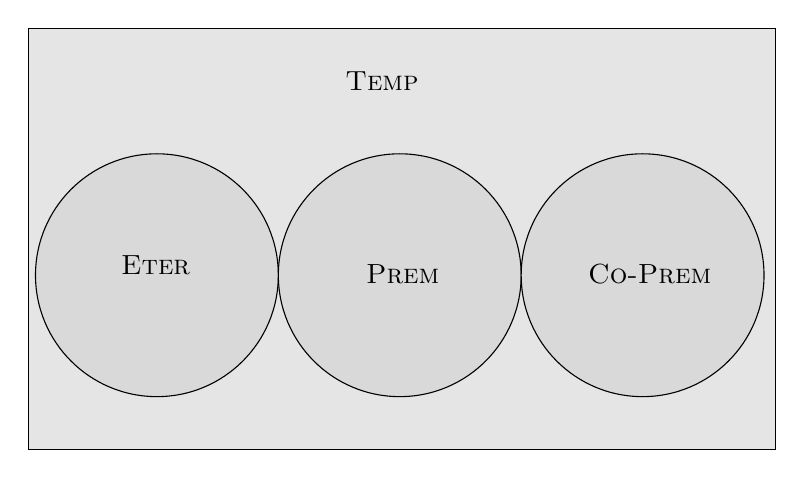
\begin{tikzpicture}[x=0.75pt,y=0.75pt,yscale=-1,xscale=1]
    %uncomment if require: \path (0,310); %set diagram left start at 0, and has height of 310

    %Shape: Rectangle [id:dp9438939353832179] 
    \draw  [fill=gray!20] (64.5,13.5) -- (424.5,13.5) -- (424.5,216.5) -- (64.5,216.5) -- cycle ;
    %Shape: Circle [id:dp6623230466810723] 
    \draw  [fill=gray!30] (68,132.5) .. controls (68,100.19) and (94.19,74) .. (126.5,74) .. controls (158.81,74) and (185,100.19) .. (185,132.5) .. controls (185,164.81) and (158.81,191) .. (126.5,191) .. controls (94.19,191) and (68,164.81) .. (68,132.5) -- cycle ;
    %Shape: Circle [id:dp16392927570144655] 
    \draw  [fill=gray!30] (185,132.5) .. controls (185,100.19) and (211.19,74) .. (243.5,74) .. controls (275.81,74) and (302,100.19) .. (302,132.5) .. controls (302,164.81) and (275.81,191) .. (243.5,191) .. controls (211.19,191) and (185,164.81) .. (185,132.5) -- cycle ;
    %Shape: Circle [id:dp6100961383336985] 
    \draw  [fill=gray!30] (302,132.5) .. controls (302,100.19) and (328.19,74) .. (360.5,74) .. controls (392.81,74) and (419,100.19) .. (419,132.5) .. controls (419,164.81) and (392.81,191) .. (360.5,191) .. controls (328.19,191) and (302,164.81) .. (302,132.5) -- cycle ;

    % Text Node
    \draw (108,122) node [anchor=north west][inner sep=0.75pt]   [align=center] {\textsc{Eter}};
    % Text Node
    \draw (226,126) node [anchor=north west][inner sep=0.75pt]   [align=center] {\textsc{Prem}};
    % Text Node
    \draw (333,126) node [anchor=north west][inner sep=0.75pt]   [align=center] {\textsc{Co-Prem}};
    % Text Node
    \draw (216,33) node [anchor=north west][inner sep=0.75pt]   [align=center] {\textsc{Temp}};


  \end{tikzpicture}
  \label{fig:venn}
\end{figure}


\chapter{Events}

Up until now, we have only considered \textit{states} in our representation using $Log_A S$. However, states alone cannot represent certain situations, such as the distinction between the following two sentences:

\begin{enumerate}[label=(\arabic*)]
    \item I ate an apple.
    \item I was eating an apple.
\end{enumerate}

\begin{equation}
    \textsc{HoldsAt}(\textsc{Ate}(I, \textsc{Apple}), t_1, t_2)
    \label{eq:ate}
\end{equation}
Sentence (1) uses the perfective aspect and presents the situation as a complete, finished event, while sentence (2) uses the imperfective aspect and focuses on the ongoing nature of the situation without indicating whether it has ended.

To represent events, we need to extend our language. Equation~\ref{eq:ate} represents a state, but we need to represent an event, so we need to introduce events into our language
which we will call $Log_A T$.

\section{Tokens and Categories of Events}
\subsection{Event Tokens}

In contrast to states, event tokens do not hold homogeneously over time.
Instead, they occur as complete wholes.
To capture this notion, we introduce a new sort $\mathcal{ET}$ for event tokens and a new function $\textsc{Occurs}$ that relates events to the time they occur.

\begin{defn}
    The function $\textsc{Occurs}: \mathcal{ET} \times \mathcal{T} \times \mathcal{T} \to \textsc{Eter}$ maps an event token,
    a starting time, and an ending time to an eternal state.
\end{defn}

\begin{defn}
    \textlbrackdbl $\textsc{Occurs}(\tau_1, \tau_2, \tau_3)$\textrbrackdbl$^{\mathcal{V}}$ = $\mathfrak{o}$(\textlbrackdbl $\tau_1$\textrbrackdbl$^{\mathcal{V}}$, \textlbrackdbl $\tau_2$\textrbrackdbl$^{\mathcal{V}}$, \textlbrackdbl$\tau_3$\textrbrackdbl$^{\mathcal{V}}$)
\end{defn}

The occurrence of an event is eternal, meaning that if an event occurred between two time points, it will always have occurred between those two time points. Additionally, each occurrence is unique, meaning that an event token occurs only once. This is captured by the following axiom:

To ensure that an event token occurs only once between any two time points, we add the following axiom.

\begin{axiom}
    \begin{equation}
        \mathfrak{o}(e, t_1, t_2) \cdot \mathfrak{o}(e, t_3, t_4) = \bot  \ if \ t_1 \neq t_3 \ or \  t_2 \neq t_4
    \end{equation}
    \label{ax:occurs_once}
\end{axiom}

Intuitively, $\mathfrak{o}(e_1, t_1, t_2)$ means that the event token $e$ occurs at some time between $t_1$ and $t_2$. We also add an axiom to ensure that an event token occurring between $t_1$ and $t_2$ is followed by $t_2$:

\begin{axiom}
    \begin{equation}
        \mathfrak{o}(e, t_1, t_2) \cdot (t_2 < t_1) = \bot
    \end{equation}
\end{axiom}

\begin{theorem} Events are heterogeneous.
    \begin{equation}
        \mathfrak{o}(e, t_1, t_2) \leq \prod_{t_3, t_4 \in \mathcal{T}} [(t_3 < t_2) \cdot (t_4 < t_1)
            \leq - \mathfrak{o}(e, t_3, t_4)].
        \label{eq:events_heterogeneous}
    \end{equation}
\end{theorem}
\begin{theorem}
    \begin{equation}
        \mathfrak{o}(e, t_1, t_2) \leq \prod_{t_3, t_4 \in \mathcal{T}} [(t_3 < t_1) \cdot (t_2 < t_4)
            \leq - \mathfrak{o}(e, t_3, t_4)].
        \label{eq:events_heterogeneous2}
    \end{equation}
\end{theorem}

Both Equation~\ref{eq:events_heterogeneous} and Equation~\ref{eq:events_heterogeneous2} follows from the
axiom~\ref{ax:occurs_once}.

That means that if an event occurs over some interval, it cannot occur over any super or sub-interval.
We think of the interval as the smallest part the event can fit in.\footnote{Allen \cite{allen1984towards} defines events in a similar way, if an event occurs over some interval, it cannot occur over any sub-interval.
}

\subsection{Event Categories}
We can easily recognize that some event token is \textit{eating an apple}. So we will add this notion of \textit{category}\footnote{VEL has a similar notion called \textit{event radicals} \cite{bennett2001unifying}} to our language.

Let $\mathcal{EC}$ be the set of event categories. We will use the following function to relate event tokens to event categories.

\[
    \textsc{Cat}: \mathcal{ET} \times \mathcal{EC} \to \mathcal{S}
\]

\begin{defn}
    \textlbrackdbl $\textsc{Cat}(\tau_1, \tau_2)$\textrbrackdbl$^{\mathcal{V}}$ = $\mathfrak{c}$(\textlbrackdbl $\tau_1$\textrbrackdbl$^{\mathcal{V}}$, \textlbrackdbl $\tau_2$\textrbrackdbl$^{\mathcal{V}}$)
\end{defn}

Unlike $\textsc{Occurs}$, $\textsc{Cat}$ does not always return eternal states.

//TODO: add justification for this.
%%TODO: add justification for this.

An event token can belong to multiple categories, thus $\textsc{Cat}$ is a many-to-many relation,a as for example an event of
\textit{driving} can be an event of \textit{commuting} at the same time.

\section{Punctual and Durative Events}

The sort $\mathcal{ET}$ for event tokens is partitioned into two subsets: $\mathcal{ET}_d$ for durative events and $\mathcal{ET}_p$ for punctual events.
Similarly, the set of event categories $\mathcal{EC}$ is partitioned into $\mathcal{EC}_d$ and $\mathcal{EC}_p$.

Punctual events is the \textit{onset} or \textit{cessation} of some state. On the other hand, a durative event is made up
of the punctual event event of some state starting to hold, the state's holding for some time, and the punctual event of the state ceasing.

A state may be associated with event categories $\uparrow s$ and $\downarrow s$ for the onset and cessation of the state, respectively.

\begin{defn}
    \begin{equation}
        \textsc{Onset} : \textsc{Perm} \cup \textsc{Temp} \to^{into} \mathcal{EC}_p
    \end{equation}
\end{defn}
\begin{defn}
    \begin{equation}
        \textsc{Cease} : \textsc{Co-Perm} \cup \textsc{Temp} \to^{into} \mathcal{EC}_p
    \end{equation}
\end{defn}

\begin{defn}
    \[
        \textlbrackdbl \textsc{Onset}(\tau)\textrbrackdbl^{\mathcal{V}}
        = \uparrow(\textlbrackdbl \tau \textrbrackdbl^{\mathcal{V}})
    \]
\end{defn}
\begin{defn}
    \[
        \textlbrackdbl \textsc{Cease}(\tau)\textrbrackdbl^{\mathcal{V}}
        = \downarrow(\textlbrackdbl \tau \textrbrackdbl^{\mathcal{V}})
    \]

\end{defn}

Intuitively, $\uparrow s$ is equivalent to $\downarrow(-s)$, and $\downarrow s$ is equivalent to $\uparrow(-s)$, Let's add the following axioms to our theory.
\begin{axiom}
    \begin{equation}
        \mathfrak{c}(e_p, \uparrow s) \cdot (\mathfrak{c}(e_p, \downarrow(- s))) = \top.
    \end{equation}
\end{axiom}
\begin{axiom}\label{ax:cessation}
    \begin{equation}
        \mathfrak{c}(e_p, \downarrow s) \cdot (\mathfrak{c}(e_p, \uparrow(- s))) = \top.
    \end{equation}
\end{axiom}

Using the above axioms, we can prove the following theorem which suggests that the arrow flip with each negation.

\begin{theorem}\label{thm:arrow_flip}
    \begin{equation}
        \mathfrak{c}(e_p, \uparrow s) \cdot \mathfrak{c}(e_p, \downarrow (-- s)) = \top.
    \end{equation}
\end{theorem}
\begin{theorem}
    \begin{equation}
        \mathfrak{c}(e_p, \downarrow s) \cdot \mathfrak{c}(e_p, \uparrow (-- s)) = \top.
    \end{equation}
\end{theorem}

Both axioms and theorems above are not enough to tell how the occurrence of onsets and cessations are related to states.
Intuitively, any
transition is immediately preceded by a state and immediately followed by its complement (or vice versa).

\begin{axiom}\label{ax:transition}
    \begin{equation}
        \mathfrak{o}(e_p, t_1, t_2) \cdot \mathfrak{c}(e_p, \uparrow s) \leq \sum_{t_3, t_4 \in \mathcal{T}}[(t_2 < t_3) \cdot \mathfrak{h}(s, t_3, t_4)]
    \end{equation}
\end{axiom}
\begin{axiom}
    \begin{equation}
        \mathfrak{o}(e_p, t_1, t_2) \cdot \mathfrak{c}(e_p, \uparrow s) \leq \sum_{t_3, t_4 \in \mathcal{T}} [(t_4 < t_1) \cdot \mathfrak{h}(-s, t_3, t_4)]
    \end{equation}
\end{axiom}

The above axioms was for the onset of a state. We can similarly prove theorems for the cessation of a state.

\begin{theorem}\label{thm:cessation}
    \begin{equation}
        \mathfrak{o}(e_p, t_1, t_2) \cdot \mathfrak{c}(e_p, \downarrow s) \leq \sum_{t_3, t_4 \in \mathcal{T}}[(t_2 < t_3) \cdot \mathfrak{h}(s, t_3, t_4)]
    \end{equation}
\end{theorem}
\begin{theorem}\label{thm:cessation_2}
    \begin{equation}
        \mathfrak{o}(e_p, t_1, t_2) \cdot \mathfrak{c}(e_p, \downarrow s) \leq \sum_{t_3, t_4 \in \mathcal{T}} [(t_4 < t_1) \cdot \mathfrak{h}(-s, t_3, t_4)]
    \end{equation}
\end{theorem}

\begin{proof}
    \begin{align*}
        \mathfrak{o}(e_p, t_1, t_2) \cdot \mathfrak{c}(e_p, \downarrow s)                                                                                     \\
         & = \mathfrak{o}(e_p, t_1, t_2) \cdot \mathfrak{c}(e_p, \uparrow (-s))  \hspace{0.29\linewidth  }  \text{Axiom~\ref{ax:cessation}}                   \\
         & \leq \sum_{t_3, t_4 \in \mathcal{T}}[(t_2 < t_3) \cdot \mathfrak{h}(-(-s), t_3, t_4)] \hspace{0.204 \linewidth}   \text{Axiom~\ref{ax:transition}} \\
         & \leq \sum_{t_3, t_4 \in \mathcal{T}}[(t_2 < t_3) \cdot \mathfrak{h}(s, t_3, t_4)]. \hspace{0.255 \linewidth}   \text{Theorem~\ref{thm:arrow_flip}}
    \end{align*}
\end{proof}

A sufficient condition for the occurrence of onsets is that a state does not hold followed by its complement. We can capture this condition by the following axiom.

\begin{axiom}\label{ax:transition_2}
    \begin{equation}
        - \mathfrak{h}(s, t_1, t_2) \cdot \mathfrak{h}(s, t_3, t_4) \cdot (t_2 < t_3)\leq \mathfrak{o}(e_p, t_2, t_3) \cdot \mathfrak{c}(e_p, \uparrow s).
    \end{equation}
\end{axiom}

We can prove a similar theorem for the cessation of a state.

\begin{theorem}\label{thm:cessation_3}
    \begin{equation}
        \mathfrak{h}(s, t_1, t_2) \cdot - \mathfrak{h}(s, t_3, t_4) \cdot (t_2 < t_3)\leq \mathfrak{o}(e_p, t_2, t_3) \cdot \mathfrak{c}(e_p, \downarrow s).
    \end{equation}
    
\end{theorem}

\begin{proof} 
    \begin{align*}
        \mathfrak{h}(s, t_1, t_2) \cdot - \mathfrak{h}(s, t_3, t_4) \cdot (t_2 < t_3) \\
        &= \mathfrak{h}(-- s, t_1, t_2) \cdot - \mathfrak{h}(s, t_3, t_4) \cdot (t_2 < t_3) \\
        &= - \mathfrak{h}(- s, t_1, t_2) \cdot - \mathfrak{h}(s, t_3, t_4) \cdot (t_2 < t_3) \\
        &= - \mathfrak{h}(s, t_1, t_2)   \cdot \mathfrak{h}(-s, t_3, t_4) \cdot (t_2 < t_3) \\
        & \leq \mathfrak{o}(e_p, t_2, t_3) \cdot \mathfrak{c}(e_p, \uparrow - s) \hspace{0.06 \linewidth} \text{Axiom~\ref{ax:transition_2}} \\
        &\leq \mathfrak{o}(e_p, t_2, t_3) \cdot \mathfrak{c}(e_p, \downarrow s) \hspace{0.06 \linewidth}  \ \ \text{Theorem~\ref{thm:arrow_flip}}
    \end{align*}
\end{proof}

We can add more restrictions based on the type of state. For example, if you are considering
a $\textsc{Prem}$ state, we can prove once an onset happens, no other onset can happen.

\begin{theorem}
    \begin{equation}
        \mathfrak{o}(e_{p1}, t_1, t_2) \cdot \mathfrak{c}(e_p, \uparrow s^{p}) \leq 
        \prod_{\substack{e_{p2} \in \mathcal{E}_p \\ t_3, t_4 \in \mathcal{T}}}[(t_2 < t_3) \cdot \mathfrak{o}(e_{p2}, t_3, t_4) ]
        \leq - \mathfrak{c}(e_{p2}, \uparrow s^{p})
    \end{equation}
\end{theorem}

Similarly, we can do the mirror for $\textsc{Co-Perm}$ states.

\begin{theorem}
    \begin{equation}
        \mathfrak{o}(e_{p1}, t_1, t_2) \cdot \mathfrak{c}(e_p, \downarrow s^{cp}) \leq 
        \prod_{\substack{e_{p2} \in \mathcal{E}_p \\ t_3, t_4 \in \mathcal{T}}}[(t_2 < t_3) \cdot \mathfrak{o}(e_{p2}, t_3, t_4) ]
        \leq - \mathfrak{c}(e_{p2}, \downarrow s^{cp})
    \end{equation}
\end{theorem}
\chapter{Log AT}

A $Log_A$T language is a set of terms partitioned into three base syntactic types

$\sigma_S, \sigma_T, \sigma_{EC}, \sigma_{ET}$ and $ \sigma_I$.

\begin{itemize}
	\item $\sigma_S$ is the set of terms denoting states.
	\item $\sigma_T$ is the set of terms denoting time points.
	\item $\sigma_{EC}$ is the set of terms denoting event categories.
	\item $\sigma_{ET}$ is the set of terms denoting event tokens.
	\item $\sigma_I$ is the set of terms denoting anything else.
\end{itemize}


\section{Syntax}
%%%%%%%%%%%%%%%%%%%%%%%%%%%%%%%%%%%%%%%%%%%%%%%%%%
%%%%%%%%%%%%%%%%%%%%%%%%%%%%%%%%%%%%%%%%%%%%%%%%%%
% \[
% 	\sqsubseteq \in \sigma_T \to \sigma_T \to \sigma_S
% \]

% \[
% 	 \sqsubset \in \sigma_T \to \sigma_T \to \sigma_S
% \]

% \[
% 	\supset \subset \in \sigma_T \to \sigma_T \to \sigma_S
% \]
\begin{itemize}

	\item
	      \[
		      \textsc{Occurs} \in \sigma_{ET} \to \sigma_T \to \sigma_T \to \sigma_S
	      \]

	\item
	      \[
		      \textsc{Cat} \in \sigma_{ET} \to \sigma_{EC} \to \sigma_S
	      \]

	\item
	      \[
		      \textsc{Onset} \in \sigma_S \to \sigma_{EC}
	      \]

	\item
	      \[
		      \textsc{Cease} \in \sigma_S \to \sigma_{EC}
	      \]

	\item
	      \[
		      \textsc{Clos} \in \sigma_{ET} \to \sigma_{ET} \to \sigma_{ET}
	      \]

	\item
	      \[
		      \textsc{Po} \in \sigma_S \to \sigma_{EC}
	      \]

	\item
	      \[
		      \textsc{Prog} \in \sigma_{EC} \to \sigma_S
	      \]
	\item \[
		      \textsc{Complete} \in \sigma_{ET} \to \sigma_S
	      \]
	\item \[
		      \textsc{Int} \in \sigma_{ET} \to \sigma_S
	      \]
\end{itemize}
%%%%%%%%%%%%%%%%%%%%%%%%%%%%%%%%%%%%%%%%%%%%%%%%%%%%%%%%%%%%%
%%%%%%%%%%%%%%%%%%%%%%%%%%%%%%%%%%%%%%%%%%%%%%%%%%%%%%%%%%%%%%%%%

% \[
% 	\tau_1 \sqsubseteq \tau_2 \in L_{\Omega}
% \]
% where $\tau_1, \tau_2 \in \sigma_T$.

% \[
% 	\tau_1 \sqsubset \tau_2 \in L_{\Omega}
% \]
% where $\tau_1, \tau_2 \in \sigma_T$.

% \[
% 	\tau_1 \supset \subset \tau_2 \in L_{\Omega}
% \]
% where $\tau_1, \tau_2 \in \sigma_T$.

\[
	\textsc{Occurs}(\tau_1, \tau_2, \tau_3) \in L_{\Omega}
\]
where $\tau_2, \tau_3 \in \sigma_T$  and $\tau_1 \in \sigma_{ET}$.

\[
	\textsc{Cat}(\tau_1, \tau_2) \in L_{\Omega}
\]
where $\tau_1 \in \sigma_{ET}$ and $\tau_2 \in \sigma_{EC}$.

\[
	\textsc{Onset}(\tau) \in L_{\Omega}
\]
where $\tau \in \sigma_S$.

\[
	\textsc{Cease}(\tau) \in L_{\Omega}
\]
where $\tau \in \sigma_S$.

\[
	\textsc{Clos}(\tau_1, \tau_2) \in L_{\Omega}
\]
where $\tau_1, \tau_2 \in \sigma_{ET}$.

\[
	\textsc{Po}(\tau) \in L_{\Omega}
\]
where $\tau \in \sigma_S$.

\[
	\textsc{Prog}(\tau) \in L_{\Omega}
\]

where $\tau \in \sigma_{EC}$.

\[
	\textsc{Complete}(\tau) \in L_{\Omega}
\]

where $\tau \in \sigma_{ET}$.

\[
	\textsc{Int}(\tau) \in L_{\Omega}
\]

where $\tau \in \sigma_{ET}$.

%%%%%%%%%%%%%%%%%%%%%%%%%%%%%%%%%%%%%%%%%%%%%%%%%%%%%
%%%%%%%%%%%%%%%%%%%%%%%%%%%%%%%%%%%%%%%%%%%%%%%%%%%%%
\section{Semantics}

\begin{defn}
	A $Log_A$T structure is a tuple $\langle \mathcal{D},\mathfrak{A}, \mathfrak{h}, \mathfrak{o}, \mathfrak{c}, <
		\rangle$ where
\end{defn}


\begin{itemize}
	\item $\mathfrak{A}$

	\item $\mathfrak{h}$
	      % \item $\subseteq: \mathcal{T} \times \mathcal{T} \to \mathcal{S}$
	      % \begin{itemize}
	      % 	\item $(t_1 \subseteq t_2) \cdot (t_2 \subseteq t_1) = \bot$ if $t_1 = t_2$
	      % 	\item $[(t_1 \subseteq t_2) \cdot (t_2 \subseteq t_3)] + (t_1 \subseteq t_3) = t_1 \subseteq t_3$
	      % 	\item $t_1 \subseteq t_1 = \top$.
	      % \end{itemize}
	      % \item $\subset: \mathcal{T} \times \mathcal{T} \to \mathcal{S}$
	      % \item $>< : \mathcal{T} \times \mathcal{T} \to \mathcal{S}$

	\item $\mathfrak{o} : \mathcal{ET} \times \mathcal{T}^2 \to \textsc{Eter}$ where
	      \begin{itemize}
		      \item $\mathfrak{o}(e, t_1, t_2) \cdot (t_2 \prec t_1) = \bot$
		      \item $\mathfrak{o}(e, t_1, t_2) \cdot \mathfrak{o}(e, t_3, t_4) = \bot  \ if \ t_1 \neq t_3 \ or \  t_2 \neq t_4$
		            %   \item $\displaystyle \sum_{t\in T} \mathfrak{h}( \mathfrak{o}(e, t_1, t_2), t) \leq \prod_{t\in T} \mathfrak{h}( \mathfrak{o}(e, t_1, t_2), t)$
	      \end{itemize}
	\item $\mathcal{ET}$ is a set partitioned by two countable subsets $\mathcal{ET}^d$ and $\mathcal{ET}^p$.
	\item $\mathcal{EC}$ is a set partitioned by two countable subsets $\mathcal{EC}^d$ and $\mathcal{EC}^p$.
	\item $\mathfrak{c} : \mathcal{ET} \times \mathcal{EC} \to \textsc{Temp}$
	\item $\uparrow :  \textsc{Temp} \cup \textsc{Prem} \to \mathcal{EC}^p$
	\item $\downarrow :  \textsc{Temp} \cup \textsc{Co-Prem} \to \mathcal{EC}^p$
	\item $\mathfrak{cl} : \mathcal{ET}^p \times \mathcal{ET}^p \to^{\text{Onto}} \mathcal{ET}^d$
	      \begin{itemize}
		      %   \item need to model durative events and punctual events.
		      \item ($\mathfrak{o}(\mathfrak{cl}(e_1, e_2), t_1, t_4))  \cdot (\exists s, t_3, t_4)[
				            \textsc{OCpair}(e_1, e_2, s, t_1, t_2, t_3, t_4) ] = \top$
	      \end{itemize}
	\item $\mathfrak{po} : \textsc{Temp} \to \mathcal{EC}^d$
	      \begin{itemize}
		      \item $\textsc{OCpair}(e_1, e_2, s, t_1, t_2, t_3, t_4) \cdot \mathfrak{c}(\mathfrak{cl}(e_1, e_2), \mathfrak{po}(s)) = \top$.
	      \end{itemize}
	\item $\mathfrak{prog} : \mathcal{EC}^d \to \textsc{Temp}$
	      \begin{itemize}
		      \item \[
			            [
					            \textsc{OCpair}(e_1, e_2, s, t_1, t_2, t_3, t_4) \cdot \mathfrak{c}(\mathfrak{cl} (e_1, e_2), ec_d)
				            ] \leq  \mathfrak{h}(\mathfrak{prog}(ec_d), t_3, t_4)\]
	      \end{itemize}
	% \item $\mathfrak{complete} : \mathcal{ET} \to \textsc{Prem}$
	%       \begin{itemize}
	% 	      \item $\displaystyle \mathfrak{h}(\mathfrak{complete}(e), t_1, t_2) \leq
	% 		            \sum_{ t_3, t_4 \in \mathcal{T}}[\mathfrak{o}(e, t_3, t_4) \cdot (t_3 < t_2)] $
	%       \end{itemize}
	% \item $\mathfrak{int} : \mathcal{E}^{d} \to \textsc{Temp}$
	%       \begin{itemize}
	% 	      \item $\mathfrak{c}(e, \mathfrak{po}(\mathfrak{int}(e))) = \top$.
	%       \end{itemize}
\end{itemize}

\subsection{Macros}
\begin{itemize}
	\item \[\textsc{NoOcc}(ec, t_1, t_2) =_{\text{def}}\]
	      \[ -\sum_{\substack{{e \in \mathcal{ET}} \\ t_3, t_4 \in \mathcal{T}}}
		      [\mathfrak{c}(e, ec) \cdot (t_1 < t_3) \cdot (t_4 < t_2) \cdot \mathfrak{o}(e, t_3, t_4)]\]
	\item \[
		      \textsc{OCpair}(e_1, e_2, s, t_1, t_2, t_3, t_4) =_{\text{def}}
	      \]
	      \[
		      \mathfrak{c}(e_1, \uparrow s) \cdot \mathfrak{c}(e_2, \downarrow s) \cdot \mathfrak{o}(e_1, t_1, t_2) \cdot \mathfrak{o}(e_2, t_3, t_4) \cdot (t_3 < t_1) \cdot \textsc{NoOcc}(\downarrow s, t_2, t_3)
	      \]
\end{itemize}

\begin{defn}Valuation function
	\begin{itemize}
		\item  \textlbrackdbl $\textsc{Occurs}(\tau_1, \tau_2, \tau_3)$\textrbrackdbl$^{\mathcal{V}}$
		      = $\mathfrak{o}$(\textlbrackdbl $\tau_1$ \textrbrackdbl$^{\mathcal{V}}$,
		      \textlbrackdbl $\tau_2$\textrbrackdbl$^{\mathcal{V}}$, \textlbrackdbl $\tau_3$\textrbrackdbl$^{\mathcal{V}}$)

		\item  \textlbrackdbl $\textsc{Cat}(\tau_1, \tau_2)$\textrbrackdbl$^{\mathcal{V}}$
		      = $\mathfrak{c}$(\textlbrackdbl $\tau_1$ \textrbrackdbl$^{\mathcal{V}}$,
		      \textlbrackdbl $\tau_2$\textrbrackdbl$^{\mathcal{V}}$)
		\item \textlbrackdbl $\textsc{Onset}(\tau)$\textrbrackdbl$^{\mathcal{V}}$
		      = $\uparrow$(\textlbrackdbl $\tau$ \textrbrackdbl$^{\mathcal{V}}$)

		\item \textlbrackdbl $\textsc{Cease}(\tau)$\textrbrackdbl$^{\mathcal{V}}$
		      = $\downarrow$(\textlbrackdbl $\tau$\textrbrackdbl$^{\mathcal{V}}$)
		\item \textlbrackdbl $\textsc{Clos}(\tau_1, \tau_2)$\textrbrackdbl$^{\mathcal{V}}$
		      = $\mathfrak{cl}$(\textlbrackdbl $\tau_1$\textrbrackdbl$^{\mathcal{V}}$,
		      \textlbrackdbl $\tau_2$\textrbrackdbl$^{\mathcal{V}}$)
		\item \textlbrackdbl $\textsc{Po}(\tau)$\textrbrackdbl$^{\mathcal{V}}$
		      = $\mathfrak{po}$(\textlbrackdbl $\tau$\textrbrackdbl$^{\mathcal{V}}$)
		\item \textlbrackdbl $\textsc{Prog}(\tau)$\textrbrackdbl$^{\mathcal{V}}$
		      = $\mathfrak{prog}$(\textlbrackdbl $\tau$\textrbrackdbl$^{\mathcal{V}}$)
		% \item \textlbrackdbl $\textsc{Complete}(\tau)$\textrbrackdbl$^{\mathcal{V}}$
		%       = $\mathfrak{complete}$(\textlbrackdbl $\tau$\textrbrackdbl$^{\mathcal{V}}$)

	\end{itemize}
\end{defn}

\include{chapters/appendix}
\chapter*{Future Work}
\addcontentsline{toc}{chapter}{Future Work}

\section{Punctual Events}
\label{sec:punctual_events}

Punctual events are events that occur at a specific point in time. They are
either onsets or cessations of a state. However, at any given point in time,
there can be a punctual event for both the onset and the cessation of a state.
So do really need them in the language? Or can we just use time points to
represent them? This is a question that needs to be investigated further.

\section{Telicity}
\label{sec:telecity}

Telicity is a property of events that is related to the notion of completion.
An event is telic if it has a natural endpoint. For example, the event of
reading a book is telic because it has a natural endpoint, which is finishing
reading the book. On the other hand, the event of running is atelic because it
does not have a natural endpoint. The event of running can be terminated at any
point in time. The event of reading a book, however, cannot be terminated
arbitrarily. It can only be terminated when the book is finished.

The notion of telicity is important and needs to be investigated and integrated
into the language.
% \include{appendix}

\bibliographystyle{plain}
\bibliography{references}
\addcontentsline{toc}{chapter}{References}

\end{document}
